\section{BenchCouncil AIBench}
{{\footnotesize
\begin{description}[labelwidth=5em, labelsep=1em, leftmargin=*, align=left, itemsep=0.3em, parsep=0em]
  \item[date:] 2020-01-01
  \item[version:] TODO
  \item[last\_updated:] 2020-01
  \item[expired:] unknown
  \item[valid:] yes
  \item[valid\_date:] TODO
  \item[url:] \href{https://www.benchcouncil.org/AIBench/}{https://www.benchcouncil.org/AIBench/}
  \item[doi:] TODO
  \item[domain:] General
  \item[focus:] End-to-end AI benchmarking across micro, component, and application levels
  \item[keywords:]
    - benchmarking
    - AI systems
    - application-level evaluation
  \item[summary:] AIBench is a comprehensive benchmark suite that evaluates AI workloads at different levels (micro, component, application) across hardware systems-covering image generation, object detection, translation, recommendation, video prediction, etc.

  \item[licensing:] TODO
  \item[task\_types:]
    - Training
    - Inference
    - End-to-end AI workloads
  \item[ai\_capability\_measured:]
    - System-level AI workload performance
  \item[metrics:]
    - Throughput
    - Latency
    - Accuracy
  \item[models:]
    - ResNet
    - BERT
    - GANs
    - Recommendation systems
  \item[ml\_motif:]
    - General
  \item[type:] Benchmark
  \item[ml\_task:]
    - NA
  \item[solutions:] TODO
  \item[notes:] Covers scenario-distilling, micro, component, and end-to-end benchmarks.

  \item[contact.name:] Wanling Gao (BenchCouncil)
  \item[contact.email:] unknown
  \item[results.links.name:] ChatGPT LLM
  \item[fair.reproducible:] Yes
  \item[fair.benchmark\_ready:] Yes
  \item[ratings.software.rating:] 0
  \item[ratings.software.reason:] Not analyzed. 

  \item[ratings.specification.rating:] 8.0
  \item[ratings.specification.reason:] Task (plasma diagnostic classification) and real-time deployment described; system specs (FPS targets) implied but not fully quantified.

  \item[ratings.dataset.rating:] 6.0
  \item[ratings.dataset.reason:] Dataset is sensor stream-based but not shared or FAIR-documented.

  \item[ratings.metrics.rating:] 8.0
  \item[ratings.metrics.reason:] FPS and classification accuracy reported and relevant.

  \item[ratings.reference\_solution.rating:] 7.0
  \item[ratings.reference\_solution.reason:] CNN model described and evaluated, but public implementation and benchmarks are not available yet.

  \item[ratings.documentation.rating:] 6.0
  \item[ratings.documentation.reason:] Paper and Gemini doc exist, but full setup instructions and tools are still in progress.

  \item[id:] benchcouncil\_aibench
  \item[Citations:] \cite{gao2019aibenchindustrystandardinternet}
  \item[Ratings:]
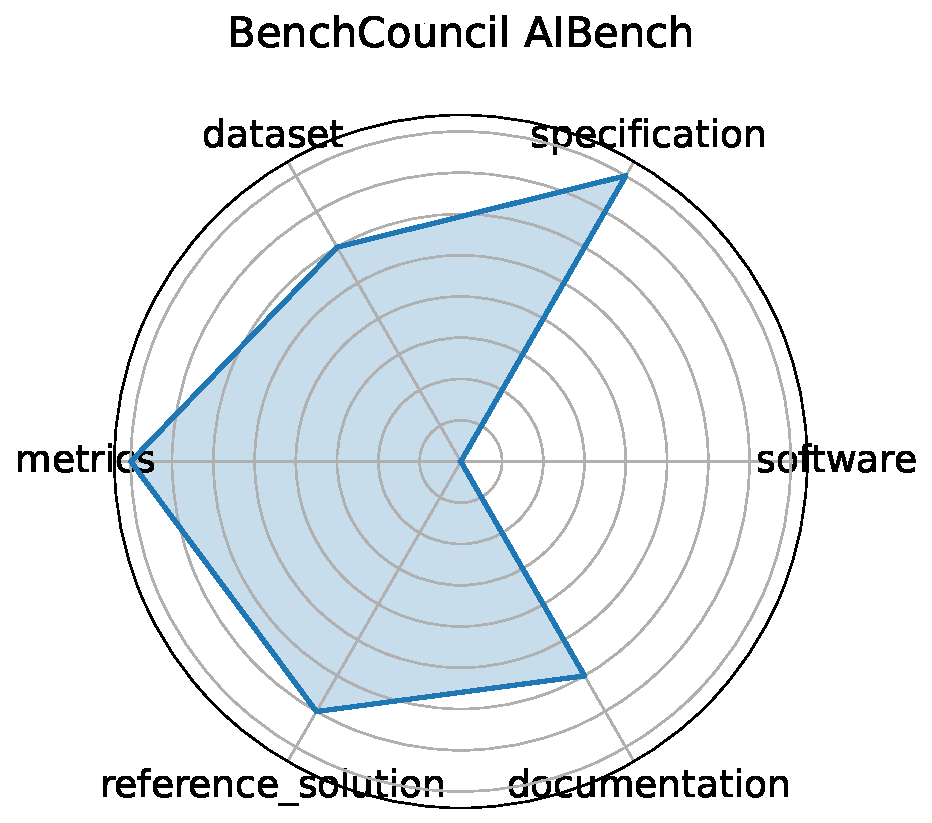
\includegraphics[width=0.2\textwidth]{benchcouncil_aibench_radar.pdf}
\end{description}
}}
\clearpage